\section{Joystick}
\begin{figure}[H]
    \centering
    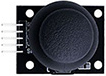
\includegraphics[angle=0, keepaspectratio=true, scale=1, width=200px, height=200px]{images/joystick.jpg}
    %\caption{Caption}
\end{figure}
\subsection*{Description}
The joystick module consists of two potentiometers (one for each axis) and a button. Each axis on the joystick has an analog output associated to it, where the output voltage is directly related to the position of the stick. The josystick can also be clicked but must be debounced.
\subsection*{Pin mapping}
This pin mapping corresponds to the pins from left to right with the module pins facing towards you.
\begin{table}[H]
    \centering
    \begin{tabular}{|c|c|c|c|c|}
    \hline
    Index &Label &Type &Name &Description\\ \hline
    0 &GND &Ground &GND &\\ \hline
    1 &+5V &Source voltage &$V+$ &Module source voltage ($5V$)\\ \hline
    2 &$\text{VR}_\text{x}$ &Analog output &A0 &Joystick x-axis output\\ \hline
    3 &$\text{VR}_\text{y}$ &Analog output &A1 &Joystick y-axis output\\\hline
    4 &SW &Digital output &D0 &Joystick switch output\\ \hline
    \end{tabular}
    %\caption{Caption}
    %\label{tab:my_label}
\end{table}
\subsection*{Operation}
The output voltage at analog pins A0 and A1 depends on the position of the joystick. Moving the joystick on either axis results in either an increase or decrease in the analog output voltage value depending on the direction it was moved. Small fluctuations caused by noise can occur when the joystick is in its resting position, so a dead-zone must be implemented to ensure correct functionality.

Clicking the joystick downwards triggers a button press which sets the digital pin D0 output to low.
\subsection*{Code}
Refer to listing \ref{python_joystick}.
%\lstinputlisting[caption=test]{laser.py}